
\documentclass[template=tabling,81pt,headonall]{azmoon}
\usepackage{xepersian}
\usepackage{amsfonts}
\usepackage{graphicx}
\graphicspath{ {./images/} }
\settextfont{Yas}
\setdigitfont{A Iranian Sans}
\usepackage{fontawesome5}

\printanswers
    \teacher{محمد صالح علی اکبری}
    \teachertitle{دبیر}
    \city{گناباد}
    \schooltitle{متوسطه دوره اول}
    \school{مقداد}
    \grade{هفتم}
    \branch{۱}
    \topic{ریاضی}
    \examdate{دی ۱۴۰۲}
    \answertime{۹۰ دقیقه}
    \begin{document}
	\begin{questions}
		\nointerlineskip%
		\vskip-\baselineskip
		\question[2.5]{%
حاصل جمع و تفریق‌های زیر را محاسبه کنید. (علامت + یا - جواب اهمیت دارد.)
    \begin{LTR}
        \begin{parts}[4]\part{$1 - 4 = $}
\part{$3 - 7 = $}
\part{$7 - 4 = $}
\part{$17 - 14 = $}
\part{$8 - 12 = $}
\end{parts}
\end{LTR}
        
    }\question[0.5]{%
میانگین بارش شهر گیسور و رحمت آباد در آذر ماه به ترتیب ۵ و ۷ میلی متر بوده است. میانگین بارش این دو شهر را محاسبه کنید. \\}\question[4]{%
حاصل جمع و تفریق‌های زیر را محاسبه کنید. (علامت + یا - جواب اهمیت دارد.)
    \begin{LTR}
        \begin{parts}[3]\part{$-223 - 57 = $}
\part{$-167 - 24 = $}
\part{$-147 - 67 = $}
‌\\‌\\\part{$-324 - 41 = $}
\end{parts}
\end{LTR}
        ‌
\\
    }\question[4]{%
حاصل تقسیم‌های زیر را محاسبه کنید.
    \begin{parts}[4]\part{ 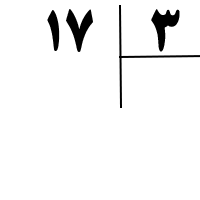
\includegraphics[scale = 0.18]{تقسیم1}}
\part{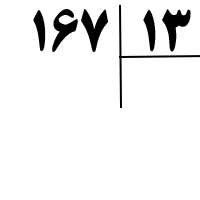
\includegraphics[scale = 0.18]{تقسیم4}}
\part{
\includegraphics[scale = 0.18]{تقسیم5}}
\part{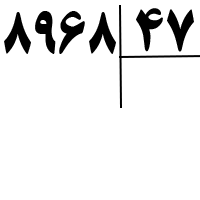
\includegraphics[scale = 0.18]{تقسیم8}}
\end{parts}
‌
\\‌
\\‌
\\
    }\question[4]{%
در $\bigcirc$ عدد علامت دار مناسب قرار دهید.
    \begin{parts}[2]\part{$-4 + \bigcirc = 5$}
\part{$-44 + \bigcirc = 75$}
\part{$14 + \bigcirc = 12$}
\part{$412 + \bigcirc = 145$}
\part{$+4 + \bigcirc = -1$}
\part{$+24 + \bigcirc = -5$}
\part{$10 + \bigcirc = 8$}
\part{$35 + \bigcirc = 17$}
\end{parts}

    }\question[1]{%
مساحت شکل زیر را محاسبه کنید. \\ 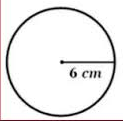
\includegraphics[scale = 0.78]{دایره با شعاع ۶} }\question[4]{%
۲ جمله بعدی دنباله‌های زیر را بنویسید و در انتها جمله nام آن را بنویسید. مانند نمونه.
    \begin{LTR}
        \begin{parts}[1]\part{$1 , 3 , 5 , 7 , 9 , 11 , 2n-1 $}
\part{$4 , 7 , 10 , .... , .... , .... , ....$}
\part{$3 , 5 , 7 , .... , .... , .... , ....$}
\part{$8 , 12 , 16 , .... , .... , .... , ....$}
\end{parts}
\end{LTR}
        
    }\end{questions}
    \end{document}
    